\documentclass{article}

% Note: Building this .tex file requires the mcode package avaialble at
% http://www.mathworks.com/matlabcentral/fileexchange/8015-m-code-latex-package

\usepackage{fullpage}
\usepackage{amsmath}
\usepackage{graphicx}
\usepackage{bm}
\usepackage{subfigure}
\usepackage[framed]{mcode}
\usepackage{color}
\usepackage{float}
\restylefloat{table}

\newcommand{\xb}{\mathbf{x}}
\newcommand{\ub}{\mathbf{u}}
\newcommand{\vb}{\mathbf{v}}
\newcommand{\zb}{\mathbf{z}}
\newcommand{\nub}{\bm{\nu}}
\newcommand{\xib}{\bm{\xib}}
\newcommand{\gammab}{\bm{\gamma}}
\newcommand{\kappab}{\bm{\kappa}}
\newcommand{\lambdab}{\bm{\lambda}}
\newcommand{\deltab}{\bm{\delta}}
\newcommand{\Ub}{\mathbf{U}}
\newcommand{\Yb}{\mathbf{Y}}
\newcommand{\hb}{\mathbf{h}}
\newcommand{\yb}{\mathbf{y}}


\author{Stephanie Tsuei}
\title{The Worst Toolbox Documentation}
\date{Version 0.1a}

\begin{document}
\maketitle

\section{Introduction}
This toolbox implements the algorithm described in:

\begin{quote}
J. E. Tierno, R. M. Murray, J. C. Doyle, and I. M. Gregory,
``Numerically Efficient Robustness Analysis of Trajectory Tracking for Nonlinear
Systems," \emph{J. Guid. Control. Dyn.}, vol. 20, no. 4, pp. 640-647, Jul.
1997.
\end{quote}

which uses theory presented in:

\begin{quote}
A. Bryson and Y. Ho, \emph{Applied optimal control: optimization,
estimation, and control}, vol. 59, no. 8. 1975.
\end{quote}



\subsection{The Robust Trajectory Tracking Problem}

\begin{figure}
\begin{center}
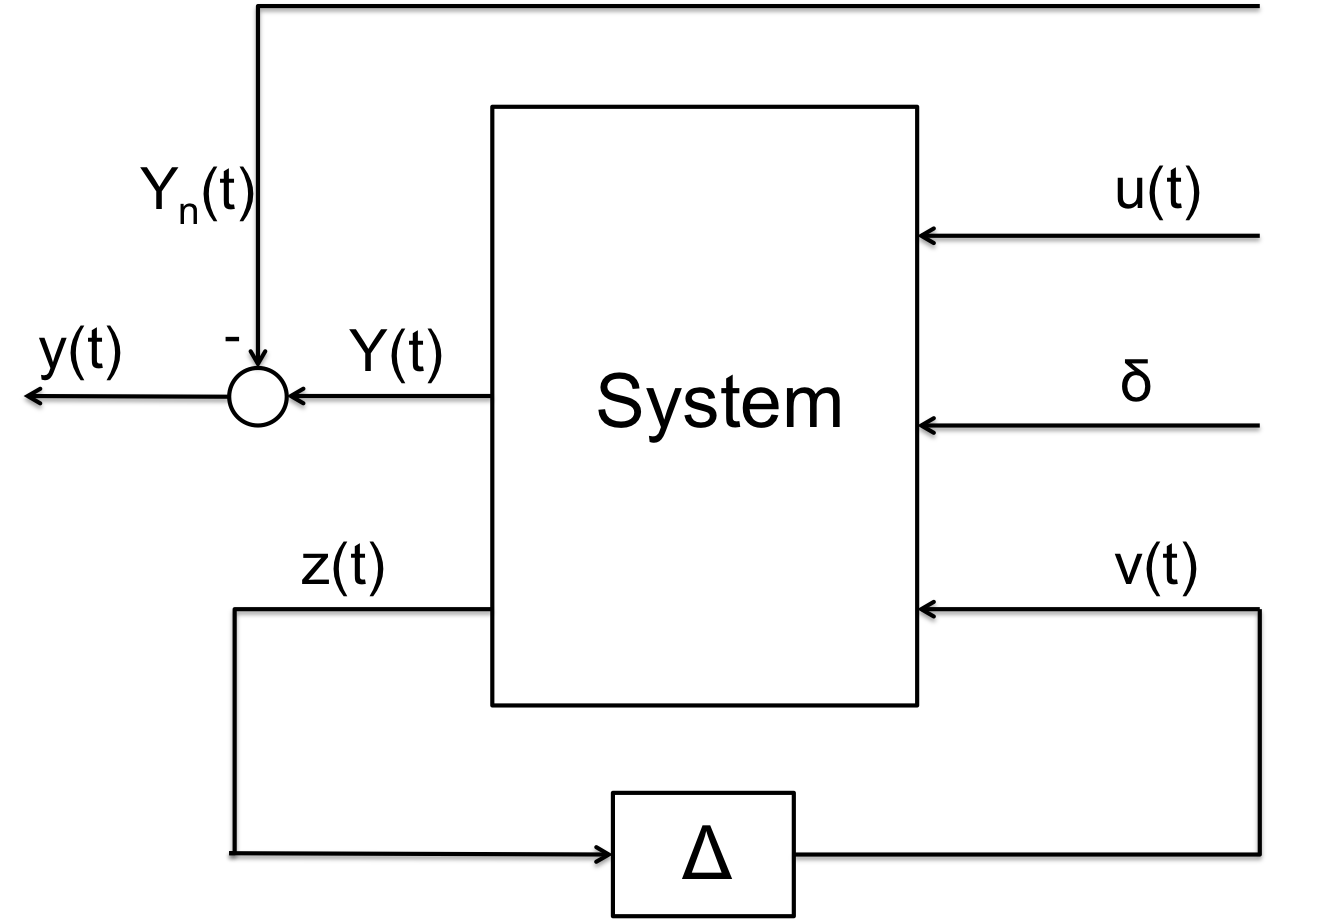
\includegraphics[width=4in]{system}
\caption{A block diagram dipicting the robust trajectory generation problem.}
\end{center}
\label{sys}
\end{figure}

Consider the dynamical system pictured in Figure \ref{sys} with dynamics
\[ \dot{\xb}(t) = f(\xb(t),\Ub(t),\ub(t),\vb(t),\deltab) \]
and outputs
\begin{align*}
\Yb(t) &= g(\xb(t),\Ub(t),\ub(t),\vb(t),\deltab) \\
\zb(t) &= h(\xb(t),\Ub(t),\ub(t),\vb(t),\deltab)
\end{align*}
where $\xb(t)$ is the state, $\Ub(t)$ is a nominal input signal, $\ub(t)$ is a
disturbance signal, $\delta$ is a vector of uncertain parameters, $\Delta$ is
an uncertain block of unit norm, and $\vb(t)$ and $\zb(t)$ are signals
representing any possible unmodeled dynamics. Therefore, the nominal
trajectory, is given by
\[ \Yb_n(t) = g(\xb(t),\Ub(t),0,0,\deltab_n) \]
where $\deltab_n$ are the nominal values of the uncertain parameters and the
quantity $\yb(t) = \Yb(t) - \Yb_n(t)$ is the error signal.


We make the following assumptions:
\begin{itemize}
	\item $\|\vb(t)\| = \|\zb(t)\|$
	\item $\vb(t)$ and $\zb(t)$ can be written in block form $\vb(t) =
	      \begin{bmatrix} \vb_1(t) & \vb_2(t) & \dots & \vb_p(t) 
		  \end{bmatrix}^T$
		  and $\zb(t) = \begin{bmatrix} \zb_1(t) & \zb_2(t) & \dots & \zb_p(t)
		  \end{bmatrix}^T$. The total number of blocks in $\vb(t)$
		  and $\zb(t)$ must be the same, but $\vb_i(t)$ and $\zb_i(t)$ can be of
		  different dimensions.
    \item $\|\ub(t)\|$ is a known constant scalar $M$ if there is only one
    	  disturbance input. If there are multiple disturbance inputs
		  $\ub_1(t)$, $\ub_2(t)$, then each disturbance input $i$ has a known 
		  norm $M_i$.
	\item $\underline{\deltab} \le \deltab_n \le \bar{\deltab}$ (elementwise) 
	      where $\underline{\deltab}$ and $\bar{\deltab}$ are known constants.
	\item We are only interested in the finite time interval $(t_i, t_f)$ and 
	      for a vector-valued time signal $\mathbf{w}(t)$, \[\|\mathbf{w}(t)\|  
		  = \left (\frac{1}{t_f-t_i} \int_{t_i}^{t_f}\mathbf{w}^T(t) 
		  \mathbf{w}(t) dt \right )^{\frac{1}{2}}\]
\end{itemize}

Given the information above, this toolbox computes the functions $\ub(t)$,
$\vb(t)$ and the value of $\deltab(t)$ that \emph{maximizes} the quantity
below: 
\[ J =  \|\yb(t)\| = \left ( \frac{1}{t_f - t_i} \int_{t_i}^{t_f} \yb(t)^T
\yb(t) dt \right )^{\frac{1}{2}}  \]

\subsection{Notes on the Algorithm} \label{algnotes}
\begin{enumerate}
\item This algorithm is a power algorithm that is not a contraction. Therefore,
it is not guaranteed to converge, but does in practice.

\item The algorithm searches for local extrema (local minima \emph{and} local
maxima). Therefore the value of $J$ that
is computed is a lower bound on the actual value of $J$.

\item Initial values for the worst case disturbance are randomly generated and
the algorithm is sensitive to the initial value of the disturbance. Therefore,
it is helpful to run the algorithm several times and plot a histogram of the
values that it computes, as seen in the examples.

\item Let $\mathbf{y}_1(t) = \begin{bmatrix}y_{1,1} (t) & y_{1,2}(t) & \dots &
y_{1,m}(t) \end{bmatrix}$ be the error output signal from the previous iteration
and $\mathbf{y}_2(t) = \begin{bmatrix} y_{2,1}(t) & y_{2,2}(t) & \dots &
y_{m,2}(t) \end{bmatrix}$ be the error output signal from the current iteration.
The algorithm declares that it has converged when \[ \max_{i = 1,2,\dots,m}
\frac{\sum_{j=1}^T (y_{1,i}(j) - y_{2,i}(j))^2}{\sum_{j=1}^T y_{1,i}(j)^2 } < e
\] where $e$ is a small positive number and $T$ is the number of timesteps.

\end{enumerate}


\subsection{System Requirements}
Requirements:
\begin{itemize}
\item Matlab R2012b or later
\item Simulink
\end{itemize}
The toolbox may work on some earlier versions of Matlab and Simulink, but was
developed on Matlab R2012b.


\subsection{Install Instructions}
To install the Worst Toolbox, place the folder \texttt{worst/} anywhere on your
local machine and add it (but not its subdirectories) to the Matlab path. This
is equivalent to the running the command:

\begin{quote}\texttt{addpath(`/path/to/robust/worst')} \end{quote}

\section{Using Worst}

\subsection{Simulink Model Configuration}
The Worst toolbox makes some assumptions about the configuration of Simulink
models:

\subsubsection*{Order of Inputs}

The program assumes that models have up to four input signals and two output
signals. Each of the signals may have arbitrary dimension to accomodate multiple
inputs, disturbances, and feedback signals. The order assumed is:
\begin{enumerate}
\item Nominal inputs, $\Ub(t)$
\item Disturbance inputs, $\ub(t)$
\item Unmodeled feedback inputs, $\vb(t)$
\item Uncertain Parameters, $\deltab$
\end{enumerate}

\subsubsection*{Order of Outputs}

Models are allowed to have an arbitrary number of outputs. If the Simulink model
has a total of $r$ outputs, and the first $m\leq r$ outputs are outputs included
in computing the performance measure $J$, then the remaining $r - m$ outputs are
unmodeled feedback outputs; the coordinates of $z$.


\subsection{Syntax of \texttt{worst}}
The syntax for \texttt{worst} is:
\begin{quote}
\texttt{worst(system\_name, output\_dimension, 'Parameter1', value1,
'Parameter2', value2, ...)}
\end{quote}
\texttt{system\_name} is the name of the Simulink model (make sure the model is
in the MATLAB path!) and \texttt{output\_dimension} is the dimension of the
system's output. The parameters are optional values, described in the table
below:

\begin{table}[H]
\begin{center}
\begin{tabular}{| c | c | p{9cm} |}
\hline
\textbf{Name} & \textbf{Default Value} & \textbf{Description} \\
\hline
\texttt{ti} & 0 & Simulation start time in seconds \\
\hline 
\texttt{tf} & 10 & Simulation end time in seconds \\
\hline
\texttt{params} & \texttt{[]} & A $p$ by 3 matrix where $p$ is the number of
uncertain scalar parameters. Each row has the format:
\texttt{[lower\_bound, nominal\_value, upper\_bound]}\\
\hline
\texttt{disturbance\_specs} & \texttt{[]} & A $d$ by 2 matrix where $d$ is the
number of disturbances. Each row has the format:

\texttt{[disturbance\_dimension, disturbance\_norm]} \\
\hline
\texttt{unmodeled\_io} & \texttt{[]} & A $b$ by 2 matrix where $b$ is the number
of unmodeled input-output pairs. The left column has all the dimensions of the
unmodeled inputs $\mathbf{v}$ and the right column has all the corresponding
dimensions of the unmodeled outputs $\mathbf{z}$.\\
\hline
\texttt{max\_iter} & 40 & The maximum number of times to iterate the algorithm
when computing a single value of $J$.\\
\hline
\texttt{error\_tol} & .01 & The value $e$ in section \ref{algnotes} \\
\hline
\texttt{num\_iter} & 10 & The number of different values of $J$ to compute. \\
\hline
\texttt{nominal\_time} & \texttt{[]} & The time axis, a column vector for the
nominal input, which is described below. \\
\hline
\texttt{nominal\_input} & \texttt{[]} & A $T$ by $q$ matrix describing the
nominal input signal, where $T$ is the length of \texttt{nominal\_time} and $q$
is the dimension of the nominal input. If a value for this parameter is
specified, then so must a value for the nominal time axis. \\
\hline
\texttt{averaging} & 1 (on) & Boolean value (0 or 1) that switches filtering on
and off. \\
\hline
\end{tabular}
\label{inputparameters}
\end{center}
\end{table}

Optional inputs whose default value is \texttt{[]} do not need to be specified
and are not necessary for the program to run. If there are no uncertain
parameters in the system, do not specify any uncertain parameters.


\subsection{Output of \texttt{worst}}
The output of \texttt{worst} is a struct containing the fields:
\begin{enumerate}
\item \texttt{converged}: A 1 by \texttt{num\_iter} array containing 0 for the
calculations that did not converge and 1 for the calculations that converged.

\item \texttt{costs}: A 1 by \texttt{num\_iter} array containing the final cost
calculated during each iteration.

\item \texttt{time\_axis}: A 1 by \texttt{num\_iter} cell array. Each entry
contains the time axis for the worst case disturbance and feedback inputs of a
computation of $\gamma$. Each time axis is a $T_i$ by 1 array, where $T_i$ is
the number of timesteps in computation $i$.

\item \texttt{v}: A 1 by \texttt{num\_iter} cell array. Each entry contains the
worst case unmodeled feedback input, an array with $T_i$ rows, from a
computation of $\gamma$. If there are multiple unmodeled feedback inputs, then
the inputs are just concatenated horizontally into one array. The time axis
entry $i$ in \texttt{v} is \texttt{time\_axis}\{i\}.

\item \texttt{d}: Same as for \texttt{v} above, except with the worst case
disturbances.

\item \texttt{p}: A 1 by \texttt{num\_iter} cell array. Each entry of the cell
array contains an array containing the worst parameter values from each
computation of $\gamma$.
\end{enumerate}


\subsection{Speeding up the Program}

\begin{figure}
\begin{center}
\subfigure[Original Simulink
Diagram]{\includegraphics[width=3.2in]{dubin\string_diagram}}
\subfigure[Diagram with 
	S-Function]{\includegraphics[width=3.2in]{dubin\string_diagram\string_sfun}}
\caption{A model of Dubin's Car compiled into an S-function.}
\end{center}
\label{sfunc}
\end{figure}

The program repeatedly calls \texttt{linmod} in order to build and simulate an
adjoint system. This greatly slows down the program because Simulink will
recompile the model with every call. To hasten computation, compile your
Simulink model into an S-function before running the program, as shown in Figure
\ref{sfunc}. The more blocks in the original Simulink model, the greater the
improvement in speed.


\section{Examples}
A few examples are below. Since compiled S-functions are not compatible across
all systems, the Simulink models of the examples are not compiled.

\subsection{A Simple Linear System}
Consider the system
\begin{gather*}
\begin{bmatrix} \dot{x}_1(t) \\ \dot{x}_2(t) \end{bmatrix} = 
	\begin{bmatrix} -3 & a \\ 2 & -5 \end{bmatrix}
	\begin{bmatrix} x_1 \\ x_2 \end{bmatrix} + 
	\begin{bmatrix} 1 \\ 2 \end{bmatrix} u(t) + 
	\begin{bmatrix} 2 \\ 1 \end{bmatrix} v(t) \\
Y(t) = x_1(t) + v(t) \\
z(t) = -x_2(t) + v(t)
\end{gather*}
where $-1 \leq a \leq 1$ is an uncertain parameter, $u(t)$ is a norm 1
disturbance, and $v(t)$ is the unmodeled feedback input. The code for the system
is below.

\lstinputlisting{../examples/linear1/linear1.m}

\subsection{A Linear System with Missing Pieces}
Consider the system
\begin{gather*}
\begin{bmatrix} \dot{x}_1 \\ \dot{x}_2 \end{bmatrix} = 
	\begin{bmatrix} -3 & a \\ 2 & -5 \end{bmatrix}
	\begin{bmatrix} x_1 \\ x_2 \end{bmatrix} +
	\begin{bmatrix} 1 \\ 2 \end{bmatrix} u(t) \\
y(t) = x_1(t)
\end{gather*}
where $-1 \leq a \leq 1$ is a scalar uncertain parameter and $u(t)$ is a
one-norm disturbance. There are no uncertain feedback loops or nominal input
signals.

\lstinputlisting{../examples/linear2/linear2.m}


\subsection{Dubin's Car}
The kinematics of Dubin's Car are
\begin{gather*}
\dot{x} = \cos(\theta) \\
\dot{y} = \sin(\theta) \\
\dot{\theta} = U(t) + u(t)
\end{gather*}
where $\begin{bmatrix} x & y & \theta \end{bmatrix}^T$ is the state, $U(t)$ is a
scalar nominal input, and $u(t)$ is a scalar disturbance with $\|u\| = 2$. The
output of the system is the full state. There are no uncertain feedback loops.

\lstinputlisting{../examples/dubin/dubincar.m}


\end{document}
